\documentclass[11pt]{article}
\usepackage[margin=2.5cm]{geometry}
\usepackage{graphicx, hyperref, tikzit}
\usepackage{amsthm, amsmath, amssymb}

\input{graphs.tikzstyles}

\geometry{
	top=1.5cm,
}

\newtheorem{theorem}{Theorem}
\theoremstyle{definition}
\newtheorem{definition}{Definition}
\theoremstyle{remark}
\newtheorem{example}{Example}
\theoremstyle{definition}
\newtheorem{proposition}{Proposition}

\hypersetup{
	colorlinks=true,
	linkcolor=blue,
	citecolor=blue,
	urlcolor=blue
}

%For urls
\usepackage{url}

\title{Model Checking Real-Time Systems\\\small Written Abstract for the Seminar ``Recent Advances in Model Checking''}
\author{Vincent Trélat}
\date{}

\begin{document}
\maketitle	

\section*{Organizational information}
% - organization of the abstract and relation to the talk
% - motivation of why the others should care
% - formalities that you plan to use in your talk
% - an outlook of what to expect in your talk 
% - if possible, a paragraph on the relation to (some of) the other talks
This abstract is based on Chapter 29 of the Handbook of Model Checking~\cite{handbook}.
Section~\ref{sec:intro} first introduces and motivates model checking applied to real-time systems, building on~\cite[Chapters~29.1 and 29.2]{handbook}.
Section~\ref{sec:ta} gives some formal definitions from ~\cite[Chapters~29.2 and 29.7]{handbook} about timed automata and discusses the reachability problem.
Section~\ref{sec:app} briefly introduces time-extended formalisms such as \emph{Timed Temporal Logic} and \emph{Timed Games}, building on~\cite[Chapters~29.6~and~29.9]{handbook}.
An additional Section~\ref{sec:lang} talks about some further material regarding language-theoretic properties that are not related to model checking and which will not be discussed in the talk.


\iffalse
Outline of the talk:
- Timed automata
- Regions
- Zones
- Timed Temporal Logics
	- LTL, continuous and pointwise semantics
	- TCTL model-checking is PSPACE-complete
- Timed Games
if time:
- Language Theoretic Properties
	- Theorems 7, 8, 9
- Branching-Time Temporal Logics
	- TCTL*, MTL
\fi



\section{Introduction}\label{sec:intro}
\paragraph{Motivation} In the early 1990s, Rajeev Alur and David Dill introduced a powerful and expressive formalism named \emph{timed automata} which have proven to be very convenient for modeling and reasoning about real-time systems.
It is nowadays a standard tool for the verification of real-time systems and has many applications in the industry, while also being a very active research area.

\paragraph{Outlook} My presentation will be based around these notions in model checking. The first is \emph{reachability}, i.e.\ given a structure, one wants to determine whether a set of locations is reachable from an initial location.
From then, we move on to richer specifications in the form of \emph{timed temporal logic} that can express various properties on timed automata.
Finally, we move on to the controller synthesis problem, which can be expressed using the formalism of \emph{timed games}.

\section{Timed Automata}\label{sec:ta}
\paragraph{Preliminaries}\label{par:prelims}
In this chapter, time values are equated with non-negative real numbers of $\mathbb{R}_{\geq 0}$. A \emph{time sequence} is a finite or infinite non-decreasing sequence of time values.
A \emph{timed word} over $\Sigma \times \mathbb{R}_{\geq 0}$ is a word over the alphabet $\Sigma$ sequentially paired with a time sequence.
%% Useless?
% If the time sequence of a timed word is upper-bounded or converging, the timed word is said to be \emph{converging} and \emph{divergent} otherwise.

Let $C$ be a finite set of variables called \emph{clocks}. A \emph{valuation} over $C$ is a mapping $v \colon C \to \mathbb{R}_{\geq 0}$. The set of valuations over $C$ is denoted $\mathbb{R}_{\geq 0}^C$ and $\text{\bf 0}_C$ denotes the valuation assigning 0 to every clock of C.

For any valuation $v$ and any time value $t$, the valuation $v + t$ denotes the valuation obtained by shifting all values of $v$ by $t$. For any subset $r$ of $C$, $v[r]$ is the valuation obtained by resetting all clocks of $r$ in $v$ to $0$.

A \emph{constraint} $\varphi$ over $C$ is recursively defined by the following grammar:
\begin{equation*}
	\varphi ::= x \odot k\ |\ \varphi \land \varphi
\end{equation*}
where $x\in C$, $k \in \mathbb{Z}$ and $\odot \in \{<, \leq, =, \geq, >\}$.
The set of constraints over $C$ is denoted by $\Phi(C)$.
We say that a valuation $v$ over $C$ satisfies $x \odot k$ when $v(x) \odot k$, and when $v$ satisfies a constraint $\varphi$, we write $v \models \varphi$. The set of valuations satisfying a constraint $\varphi$ is denoted by $[\![\varphi]\!]_C$.

% There exists an extension to $x - y \odot k$ constraints called diagonal constraints, and the set of diagonal constraints is denoted $\Phi_d(C)$.

\paragraph{Timed Automata}\label{par:ta}
A timed automaton is basically a finite automaton with (real-time) constraints on the states.
The following formal definition is a reformulation of~\cite[Chapter 29.2, Definition 1]{handbook}.
\begin{definition}\label{def:ta}
	A \emph{Timed Automaton} (TA) $A$ is the tuple $(L, \ell_0, C, \Sigma, I, E)$ where
	$L$ is a finite set of \emph{locations} with initial location $\ell_0 \in L$,
	$C$ is a finite set of \emph{clocks},
	$\Sigma$ is a finite set of \emph{actions},
	$I \colon L \to \Phi(C)$ is an \emph{invariant mapping} and
	$E \subseteq L \times \Phi(C) \times \Sigma \times 2^{C} \times L$ is a set of edges.

	Any edge $(\ell, \varphi, a, r, \ell') \in E$ is denoted by $\ell \xrightarrow{\varphi, a, r} \ell'$ where $\varphi$ is a \emph{guard}, and $r$ is a subset of clocks that are set to zero after taking the transition.
\end{definition}
An example consisting of the graphic representation of a timed automaton is given in Fig.~\ref{fig:ta_ex}.

\begin{figure}[ht]
\centering
\ctikzfig{fig1}
\caption{Representation of a timed automaton.}\label{fig:ta_ex}
\end{figure}

\paragraph{Semantics}\label{par:semantics}
The \emph{operational semantics} of a TA $A = (L, \ell_0, C, \Sigma, I, E)$ is the infinite-state timed transition system $[\![A]\!] = (S, s_0, \Sigma \times \mathbb{R}_{\geq 0}, T)$, where
\begin{align*}
	&S := \{(\ell, v) \in L \times \mathbb{R}_{\geq 0}^C\ |\ v \models I(\ell)\}, \quad s_0 := (\ell_0, \text{\bf 0}_C),\\
	&T := \{(\ell, v) \xrightarrow{d, a} (\ell', (v+d)[r]) \ | \ d \in \mathbb{R}_{\geq 0}, \forall d' \in [0, d], v + d' \models I(\ell) \land \exists \ell \xrightarrow{\varphi, a, r} \ell' \in E, v + d \models \varphi \}
\end{align*}

The valuation $(v+d)[r]$ is the valuation obtained by adding the value $d$ to the evaluation of $v$ on any clock -- $v$ is delayed by $d$ -- in which all clocks of $r$ are reset to $0$.

%% Informal description of the semantics:
% $S$ is the set of states | i.e.\ pairs of a location and a valuation such that the valuation is | satisfying the invariant and $s_0 := (\ell_0, \text{\bf 0}_C)$ is the inital state;
% $T$ is the set of transitions that one can take by selecting a delay to be elapsed in $\ell$ and an edge of $\mathcal{A}$ to be taken after the delay\footnote{Provided that the invariant and the guard are satisfied!}.

%% Some comments about non-Zenoness?
%% Formal definition : ``A timed automaton is non-Zeno if any finite run can be extended into a time-divergent run.''
%% ==> Zenoness informally represents nonrealizable behaviour, since their execution would require to perform infinitely many actions in finite time.

\paragraph{Parallel Composition}\label{par:ta_parcomp}
It is possible to compose several TA in parallel. Informally, parallel composition roughly consists in pairing the automata w.r.t. some \emph{synchronization function} and taking the conjunction of their invariants. The point is that systems can be defined in a compositional way.

\paragraph{Region Equivalence}\label{par:ta_regeq}
Informally, two valuations are region equivalent if a TA cannot differentiate between them and we write\footnote{$M := (M_x)_{x \in C}$ where $M_x$ is the maximal constant clock $x$ is compared to in the TA.} this relation as $\cong_M$.
More formally, two valuations are region equivalent if their evaluations on any clock have the same integral parts and one has its fractional part as zero iff the other has its fractional part as zero and the order of the fractional parts is the same among different clocks.

This notion is extended to states of the TA by defining $(\ell, v) \cong_M (\ell', v')$ iff $v \cong_M v'$ and $\ell = \ell'$. The equivalence class of $(\ell, v)$ is denoted $[\ell, v]_{\cong_M}$.
As an example, we give a representation of clock regions of $A$ (see Fig.~\ref{fig:ta_ex}) in Fig.~\ref{fig:ta_reg}.

\begin{figure}[ht]
	\centering
	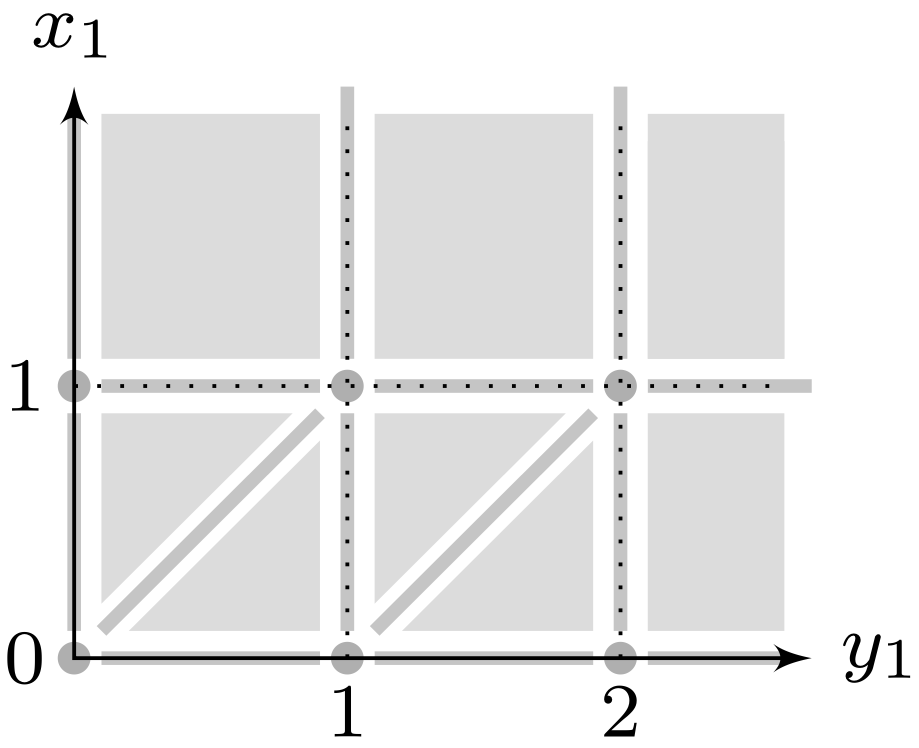
\includegraphics[width=.25\textwidth]{../img/TAreg.png}
	\caption{Graphic representation of the regions of the timed automaton $A$ given in Fig.~\ref{fig:ta_ex}.}\label{fig:ta_reg}
	\tiny{Figure taken from \cite[Chapter 29.3]{handbook}}	
\end{figure}

From this notion, we can define the \emph{region automaton} $\mathcal{R}_{\cong_M}(\mathcal{A}) = (S, s_0, \Sigma, T)$ which basically consists in quotienting $\mathcal{A}$ w.r.t.\ $\cong_M$:
$$
S = (L \times \mathbb{R}_{\geq 0})_{/\cong_M} \quad
s_0 = [\ell_0, \text{\bf 0}_C]_{\cong_M} \quad
T = \{ [\ell, v]_{\cong_M} \xrightarrow{a} [\ell', v']_{\cong_M}\ | \ \exists d, (\ell, v) \xrightarrow{d, a} (\ell', v')\}
$$

%% Non essential
% \begin{proposition}\label{prop:ta_reach}
% 	A set $F \subseteq L$ of target locations is reachable in $\mathcal{A}$ iff $S_F := \{[\ell,v]\cong_M\ |\ \ell \in F\}$ is reachable in $\mathcal{R}_{\cong_M}(\mathcal{A})$ from $s_0$.
% \end{proposition}

The region automaton $\mathcal{R}_{\cong_M}(\mathcal{A})$ is a finite automaton whose size is exponential compared with the size of $\mathcal{A}$. It can be used to check, reachability properties and ``one of the most fundamental theorems'' \cite[Chapter 29.2, Theorem 1]{handbook} states that the reachability problem (or equivalently emptiness) in TA is PSPACE-complete \cite[Section~4.5]{AlurDill}.

\paragraph{Zones} \label{par:zones}
The number of states obtained from the region partitionning is unfortunately extremely large, so the notion of \emph{zones} was introduced as a coarser representation of the state space. \emph{Zones} are exactly the sets $[\![\varphi]\!]_C$ of valuations satisfying any guard $\varphi \in \Phi_d(C)$\footnote{$\Phi_d(C)$ is the set of \emph{diagonal constraints} over $C$, i.e.\ constraints of the form $x - y \odot k$.}.
Similarly to the region automaton, we can define the \emph{zone automaton}, except that the zone automaton is infinite, so zones need to be \emph{normalized}, which basically consists in quotienting each zone w.r.t.\ the equivalence relation $\cong_M$. This operation does not produce zones in general, other operators are therefore used in practice, such as the \emph{extrapolation} of a \emph{shortest-path-closed} DBM (\emph{difference-bound matrix}).

% Any binary relation $R$ is a \emph{timed simulation} if for any two equivalent states $s_1\ R\ s_2$, and any transition $s_1 \xrightarrow{d, a} s_1'$, $s_2$ can reach a state $s_2'$ with the same transition $s_2 \xrightarrow{d, a} s_2'$ such that $s_1'\ R\ s_2'$. It is a \emph{timed bisimulation} if it is a timed simulation and symmetric.

% The relation $\cong_M$ has the weaker property of \emph{time-abstracted bisimulation}, which informally means that for a binary relation $R$ on states, from any two equivalent states the TA can take the same transitions, expect that the delays might differ.

% An important result \cite[Chapter 29.4.2]{handbook} is that decidability of both timed and time-abstracted (bi)similarity is ensured for TA.

%% Non essential
% Any two automata being timed bisimilar are also time-abstracted bisimilar.

\paragraph{Extensions}\label{par:ta_ext}
Many extensions of TA were proposed in the literature, such as allowing \emph{diagonal constraints}, \emph{updatable} TA\footnote{Clocks can be updated to any value instead of being reset to 0.} or adding \emph{urgency} requirements. However, it has been shown that such extensions are no more expressive than the original class of TA. Furthermore, most other attempted extensions generally lead to undecidability of the reachability problem, e.g.\ aadding constraints of the form $\lambda x + \mu y \leq k$ or $x := x + k$, or more complex classes such as \emph{hybrid} automata.

\section{Model checking timed systems}\label{sec:app}
\paragraph{Timed Temporal Logic}\label{par:timedlogic} We extend the usual theory of LTL presented in \cite[Chapter~2]{handbook} to timed systems with MTL (\emph{Metric Temporal Logic}).
Given a set of atomic propositions $P$, the formulas of MTL are defined for any interval $I$ with the \emph{time-constrained until} operator $\text{\bf U}_I$ as follows:
\begin{equation*}
	\varphi ::= p \in P\ |\ \neg \varphi\ |\ \varphi \land \varphi\ |\ \varphi \text{\bf U}_I \varphi
\end{equation*}
Similarly to LTL, the \emph{constrained always} operator $\square_I$ and \emph{constrained eventually} operator $\lozenge_I$ can be defined with $\text{\bf U}_I$ in this time-constrained setting. Two different semantics are usually adopted for MTL, namely the \emph{continuous} and \emph{pointwise} semantics. Informally, the pointwise semantics allows one to assert formulas only at a discrete set of points, while the continuous semantics allows one to assert formulas at arbitrary time points.

As one may imagine, bringing such expressiveness affects decidability. Although model checking and satisfiability for classical LTL are PSPACE-complete over both semantics, it is easy to see that the continuous semantics is strictly more expressive than the pointwise semantics, which results in losing decidability for model checking and satisfiability for MTL over the continuous semantics, as well as over the pointwise semantics for infinite words. By reducing expressiveness of MTL\footnote{See for instance MITL (EXPSPACE-complete), ECTL (PSPACE-complete) and MTL over \emph{bounded time} (EXPSPACE-complete).}, one can recover decidability for model checking and satisfiability over both semantics.

The case of branching-time logics such as CTL and CTL* can be adapted to timed systems as well, by means of TCTL and TCTL*. Unfortunately, only TCTL model checking is decidable (and PSPACE-complete).

\paragraph{Timed Games}\label{par:timedgames}
As explained in \cite[Chapter 27]{handbook}, games provide a convenient framework for modeling and reasoning about environments that may be affected by several (uncontrollable) agents.
An important result is that (time-optimal) reachability and safety games are decidable and EXPTIME-complete for timed games.
The key ingredient of the proof of this result is that it is sufficient for those specific control objectives to consider \emph{memoryless} strategies, i.e.\ strategies that do not depend on the history of the game.
By considering time divergent\footnote{Such an assumption stems from the condition of \emph{non-Zenoness} which is another interesting notion. Basically, a run is \emph{Zeno} if it can take infinitely many transitions in finite time.} strategies only, deciding the existence of a winning strategy for reachability and safety games is EXPTIME-complete.

Timed games can also be used to decide bisimilarity of two states of an automaton (in exponential time).
Informally, two states of a TA are time bisimilar (for some equivalence relation) if the TA can take the same transitions from those states.

Timed games have received a lot of attention recently, some work has been conducted on extensions in which, for instance, players have different objectives.

\section{Language-Theoretic Properties}\label{sec:lang}
All the above sections are related to model-checking properties of timed automata.
In this section, we present some of the most important results related to \emph{timed languages} defined over $(\Sigma \times \mathbb{R}_{\geq 0})^*$.
For instance, contrary to the untimed case, $\varepsilon$-TA are strictly more expressive than TA and one cannot decide whether a given $\varepsilon$-TA has a TA equivalent (without $\varepsilon$-transitions).
Although in the general case the language-inclusion problem -- i.e.\ deciding if $\mathcal{L}(A) \subseteq \mathcal{L}(B)$ holds for two given timed automata $A$ and $B$ -- is undecidable for TA, it may recover its decidability in some special cases, such as $B$ is an \emph{event-clock automaton} (over infinite words) or has at most one clock (over finite words), or under \emph{closed-time} or \emph{bounded-time} assumptions.

\bibliographystyle{alpha}
\bibliography{ref}

\end{document}